%\documentclass[12pt]{article}
%\usepackage[a4paper, margin=1in]{geometry} 
%\usepackage{graphicx} 
%\usepackage{hyperref}
%\usepackage{float}
%\usepackage{multicol}
%\usepackage{multirow}
%\usepackage{amsmath}
%\usepackage[table,xcdraw]{xcolor}
%\usepackage[font=small, labelfont=bf]{caption}
%
%\begin{document}

%
% HMM profile
%
\subsection{HMM profile}
An HMM (Hidden Markov model) profile is similar to a regular profile, but it is based on a probabilistic graphical model.

%
% HMM profile to find local alignments
%
\subsubsection*{HMM profile to find sub-strings}
An HMM profile represents position-specific probabilities of amino acids.

\begin{figure}[H]
  \centering
      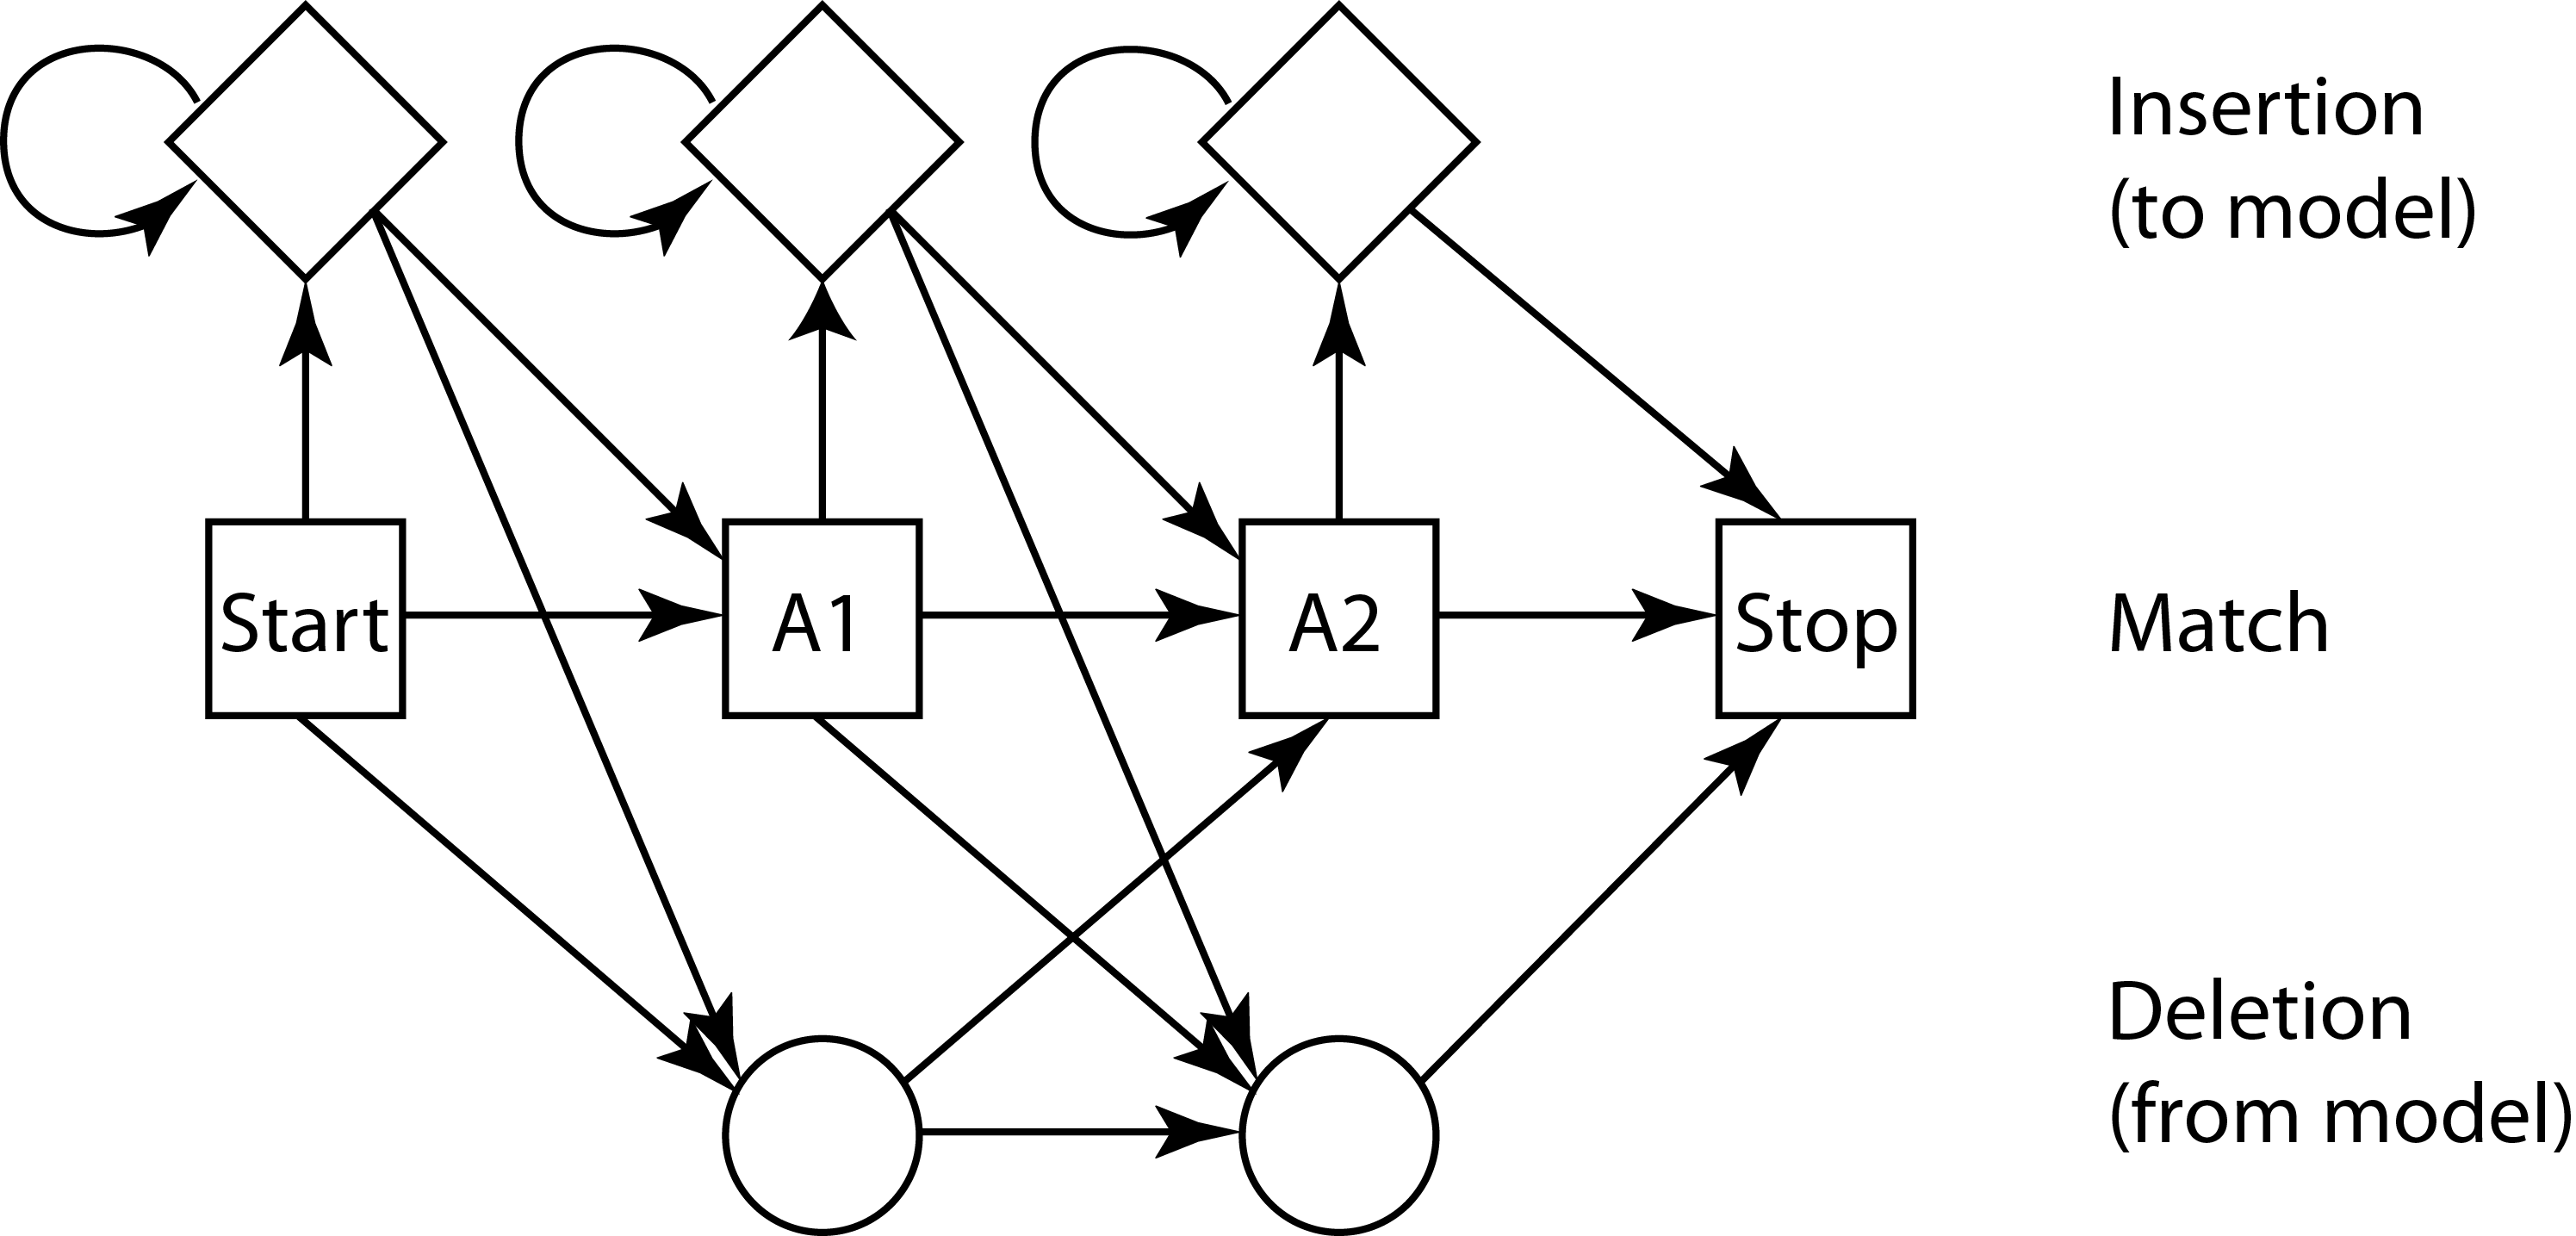
\includegraphics[width=0.5 \textwidth]{fig13/HMM_profile_example_1.png}
  \caption{An HMM for an alignment of two columns A1 and A2}
\end{figure}

%
% Example of HMM profile for finding local alignments
%
\subsubsection*{Example of HMM profile for finding sub-strings}
Assume Seq1 = ’q1 q2 q3 q4’ and its path is indicated with solid lines. Create the alignment of Seq1 and the profile.

\begin{table}[H]
\small
\centering
\begin{tabular}{|l|l|l|l|l|l|}
\hline
   & Start                    & Insertion                & Match                    & Deletion                 & Stop                     \\ \hline
   & -1                       & \cellcolor[HTML]{C0C0C0} & \cellcolor[HTML]{C0C0C0} & \cellcolor[HTML]{C0C0C0} & \cellcolor[HTML]{C0C0C0} \\ \hline
q1 & \cellcolor[HTML]{C0C0C0} & (2 start)                &                          &                          & \cellcolor[HTML]{C0C0C0} \\ \hline
q2 & \cellcolor[HTML]{C0C0C0} &                          & (4 deletion)             & (3 insertion)            & \cellcolor[HTML]{C0C0C0} \\ \hline
q3 & \cellcolor[HTML]{C0C0C0} & (5 match)                &                          &                          & \cellcolor[HTML]{C0C0C0} \\ \hline
q4 & \cellcolor[HTML]{C0C0C0} & (6 Insertion)            &                          &                          & \cellcolor[HTML]{C0C0C0} \\ \hline
   & \cellcolor[HTML]{C0C0C0} & \cellcolor[HTML]{C0C0C0} & \cellcolor[HTML]{C0C0C0} & \cellcolor[HTML]{C0C0C0} & (7 insertion)            \\ \hline
\end{tabular}
\end{table}

\begin{figure}[H]
  \centering
      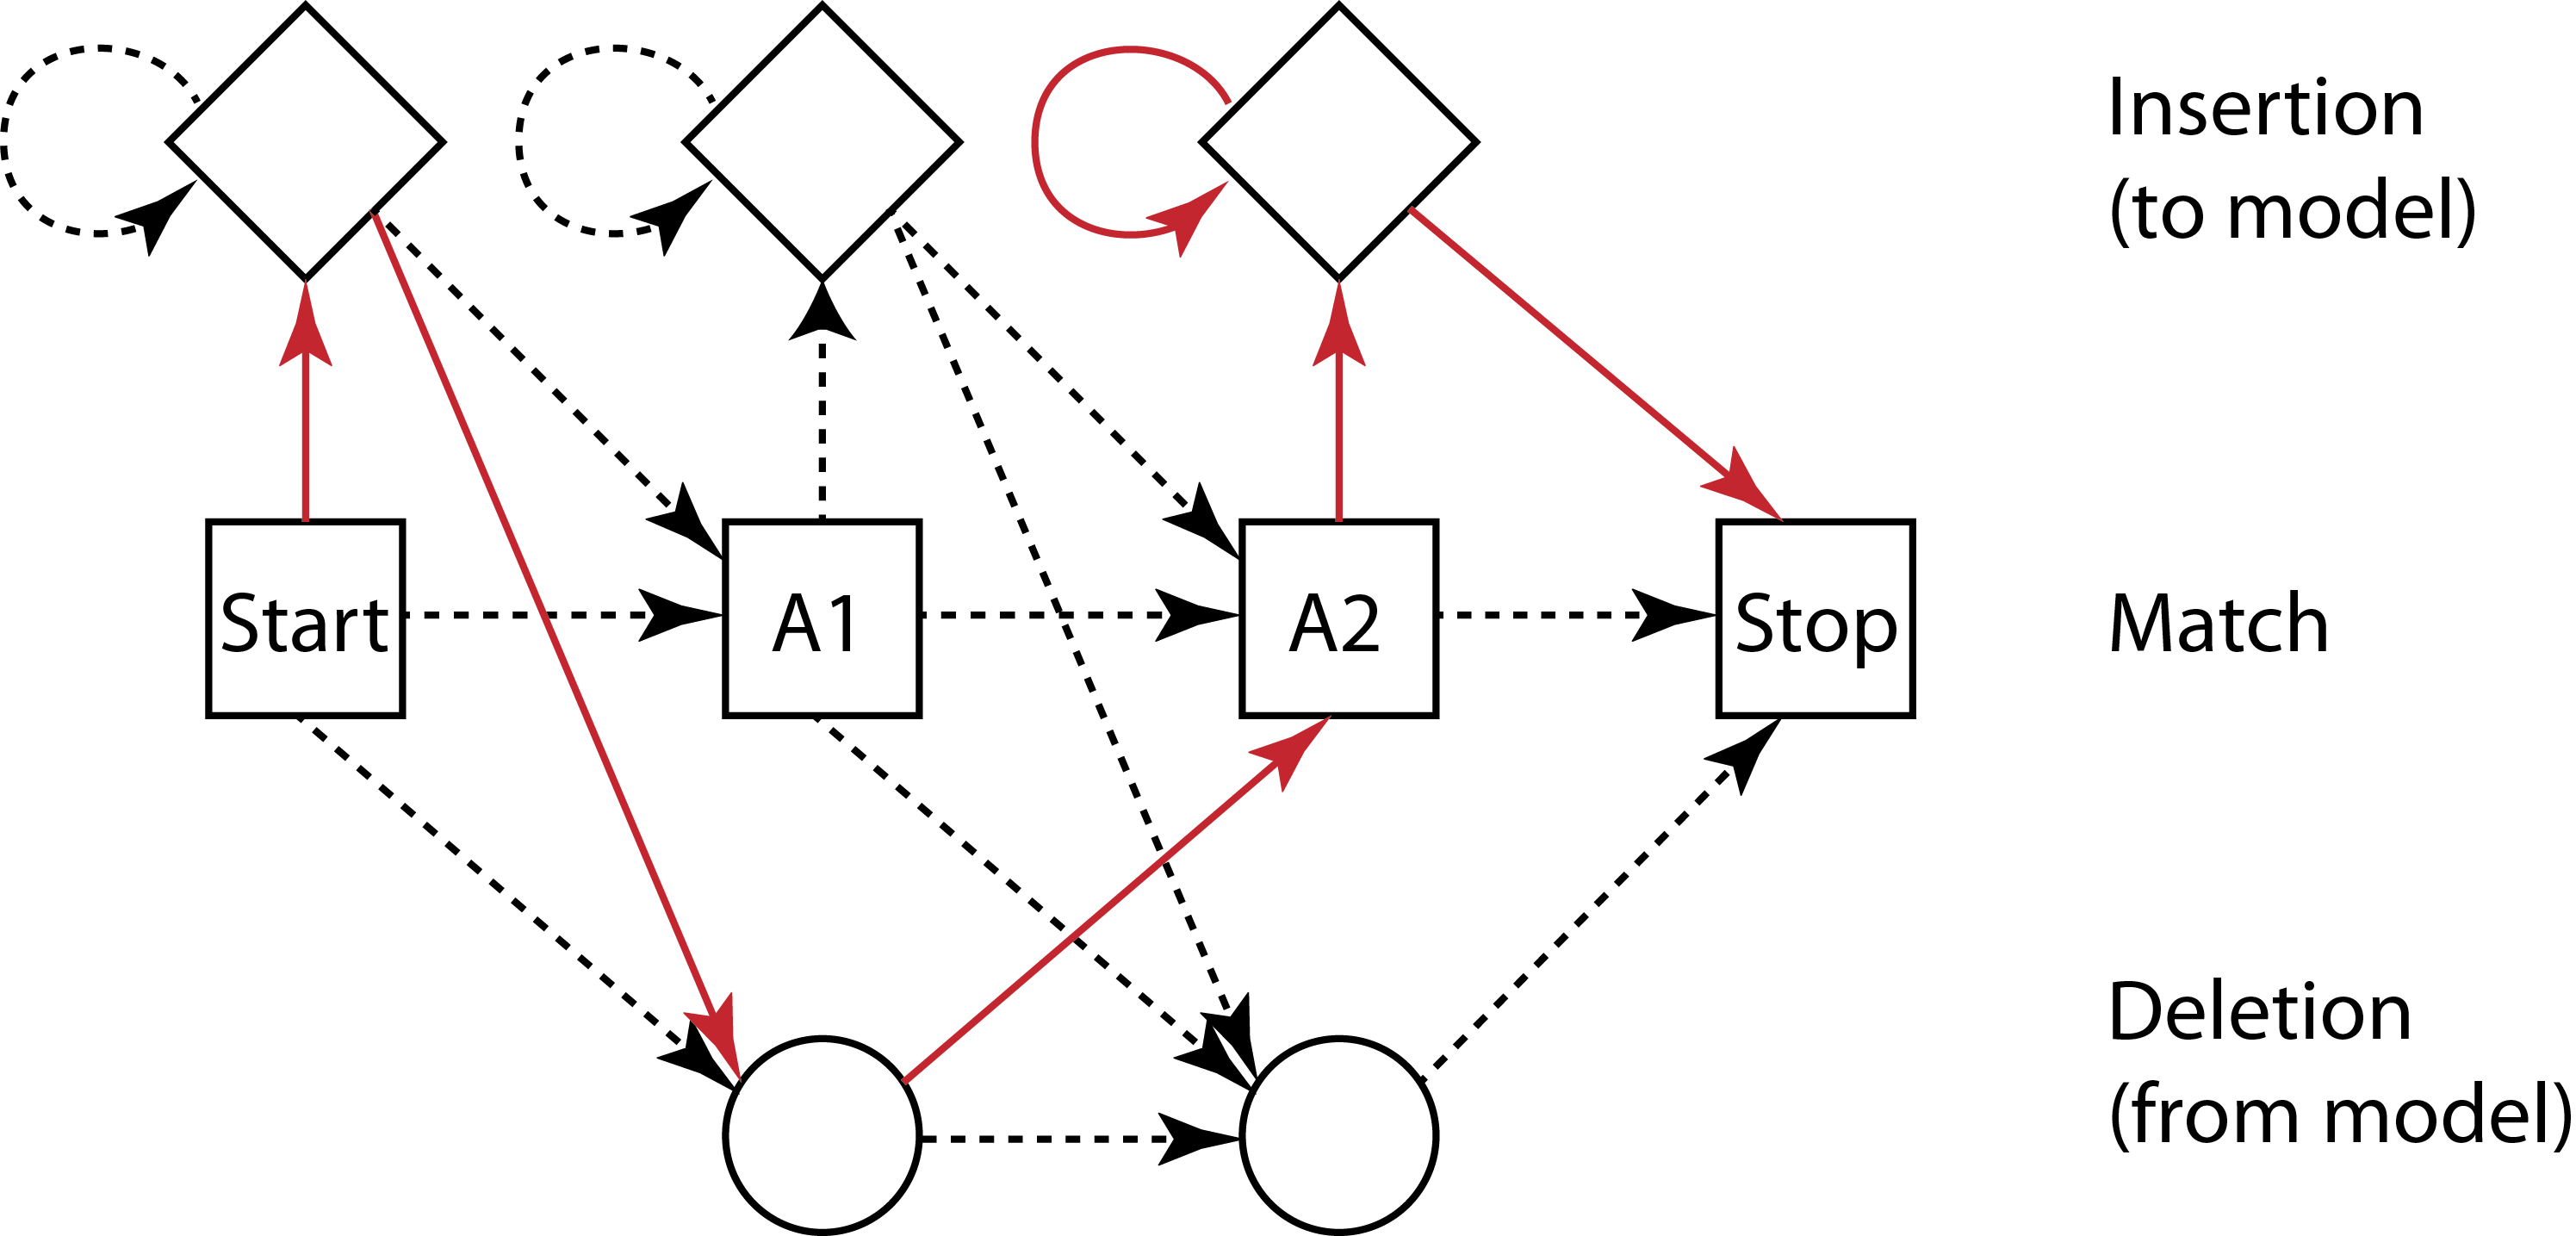
\includegraphics[width=0.5 \textwidth]{fig13/HMM_profile_example_2.png}
  \caption{An HMM profile to find the optimal alignment}
\end{figure}

\noindent
Local alignment:
\begin{verbatim}
   q1  -   q2  q3  q4
   -   A1  A2  -   -
\end{verbatim}

\bigskip 

%\end{document}
